All discussion so far involved either simulated samples, Belle~II data samples with \BtoXsgamma events negligible,
or with the signal region ($\EB\in(1.8,2.7)~\gev$) hidden.
After preparing the analysis on simulation, performing extensive validation and evaluating systematic uncertainties, 
the signal region is ready to be unblinded, as it was shown that no significant biases are expected.
This section presents the results of the analysis.

\subsection{\texorpdfstring{\Mbc}{Mbc} fit results}\label{sec:mbc_fit_results}

Following the \Mbc fitting strategy described in \Cref{sec:fitting_setup} and the model in \Cref{tab:fitting_init_params_updated},
the fits on the signal region if Belle~II data are performed.
They are shown in \Cref{fig:data_fits_signal}.
Together with fits in \Cref{fig:sideband_data_fit}, it gives all the fits for the defined \EB intervals in \Cref{sec:binning}.
The extracted $\mathcal{N}_{\mathrm{CB}}$ are shown in the top right corner of each figure.

The fit results on Belle~II simulation, with all \BtoXsgamma events removed, are shown in \Cref{fig:nosignal_fits_signal}.
The extracted number of \BB background events is shown in \Cref{fig:nosignal_fits_signal}.
These values are corrected and scaled and are equal to the ones listed in \Cref{tab:background_uncertainties}.

\begin{figure}[htbp!]
    \centering
    \subcaptionbox{\label{fig:data_fit_1p8_2p0}}{
        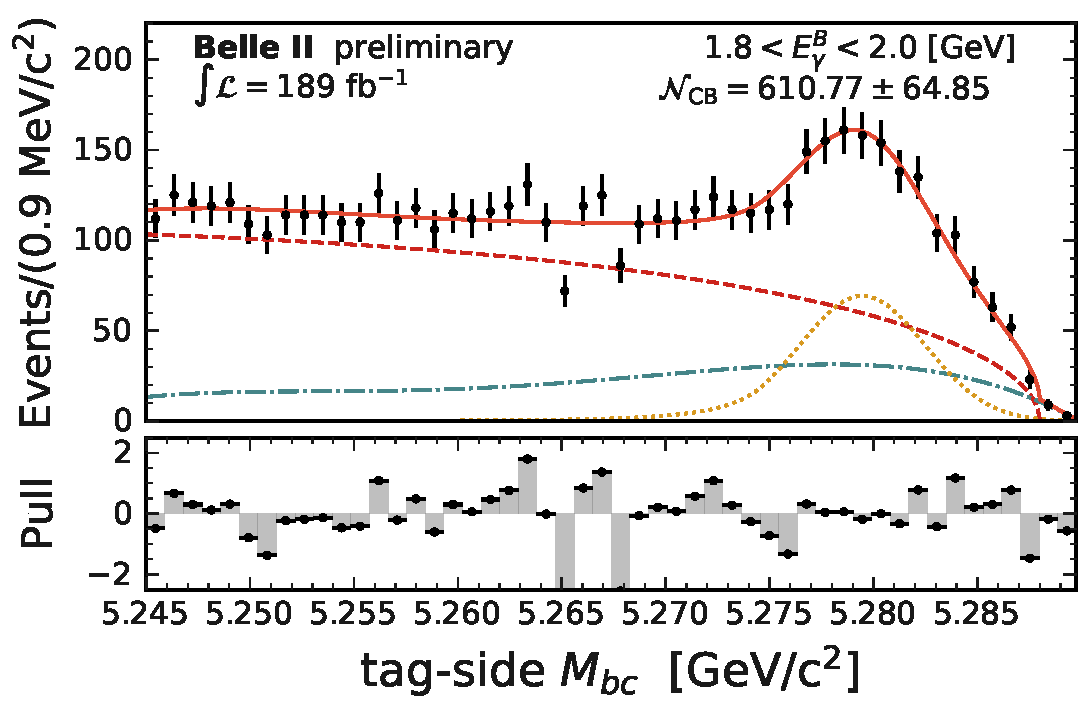
\includegraphics[width=0.3\textwidth]{figures/final_results/data_fits/DATA_MbcFit_1p8to2p0ppdf.pdf}
    }
    \subcaptionbox{\label{fig:data_fit_2p0_2p1}}{
        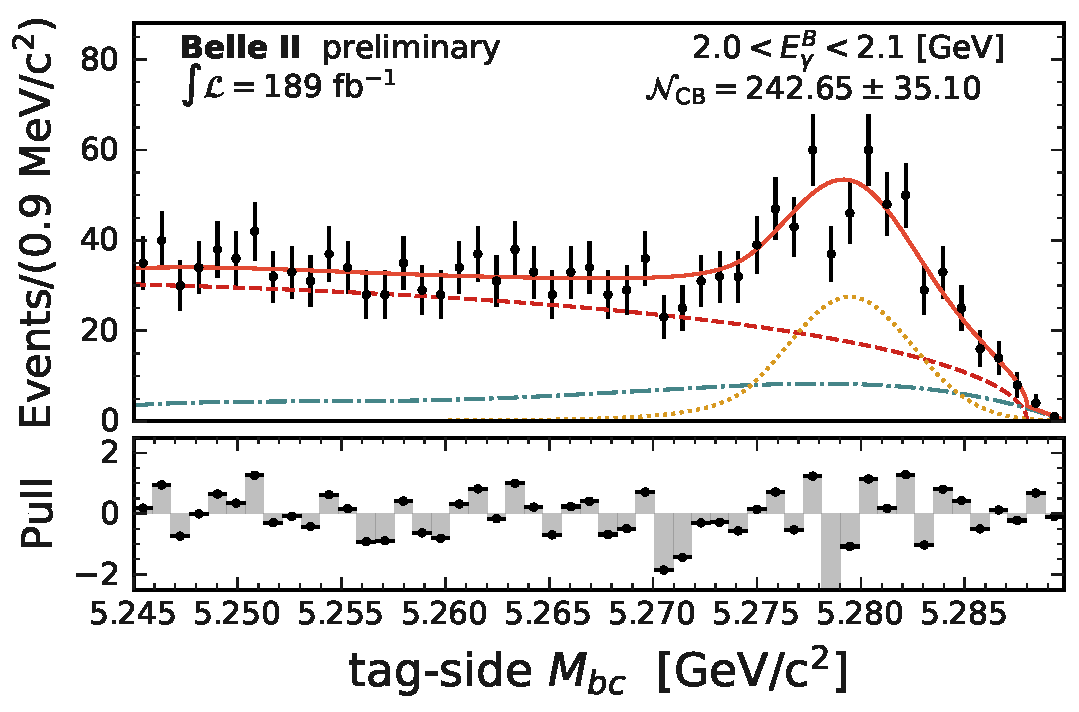
\includegraphics[width=0.3\textwidth]{figures/final_results/data_fits/DATA_MbcFit_2p0to2p1ppdf.pdf}
    }
    \subcaptionbox{\label{fig:data_fit_2p1_2p2}}{
        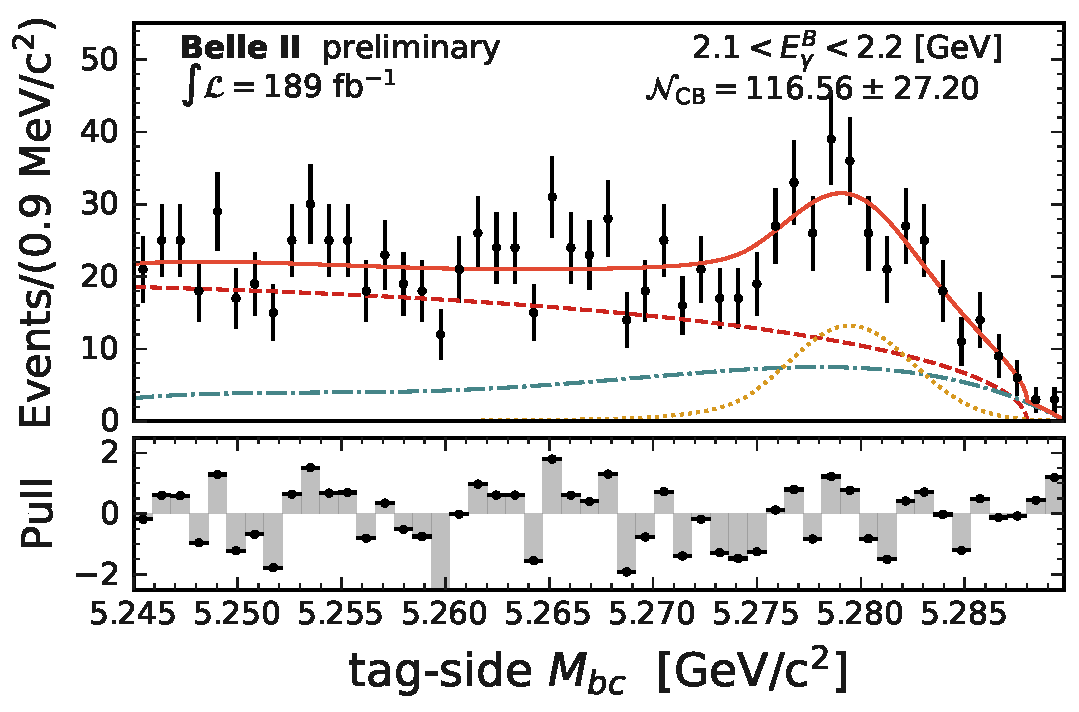
\includegraphics[width=0.3\textwidth]{figures/final_results/data_fits/DATA_MbcFit_2p1to2p2ppdf.pdf}
    }
    \subcaptionbox{\label{fig:data_fit_2p2_2p3}}{
        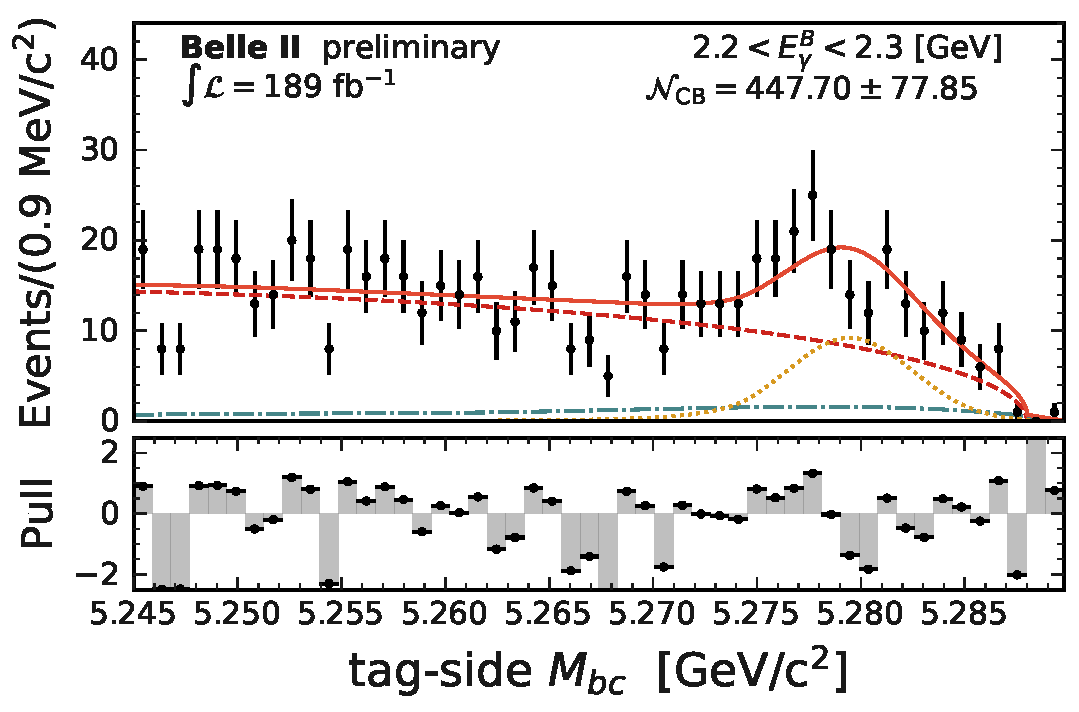
\includegraphics[width=0.3\textwidth]{figures/final_results/data_fits/DATA_MbcFit_2p2to2p3ppdf.pdf}        
    }
    \subcaptionbox{\label{fig:data_fit_2p3_2p4}}{
        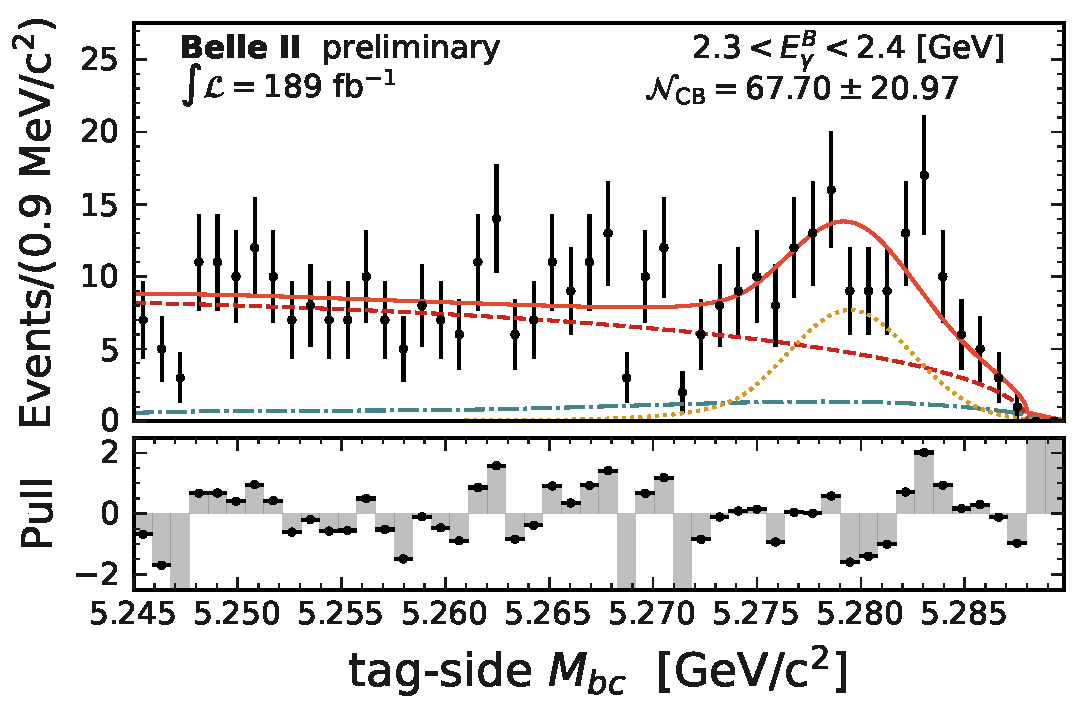
\includegraphics[width=0.3\textwidth]{figures/final_results/data_fits/DATA_MbcFit_2p3to2p4ppdf.pdf}
    }
    \subcaptionbox{\label{fig:data_fit_2p4_2p5}}{
        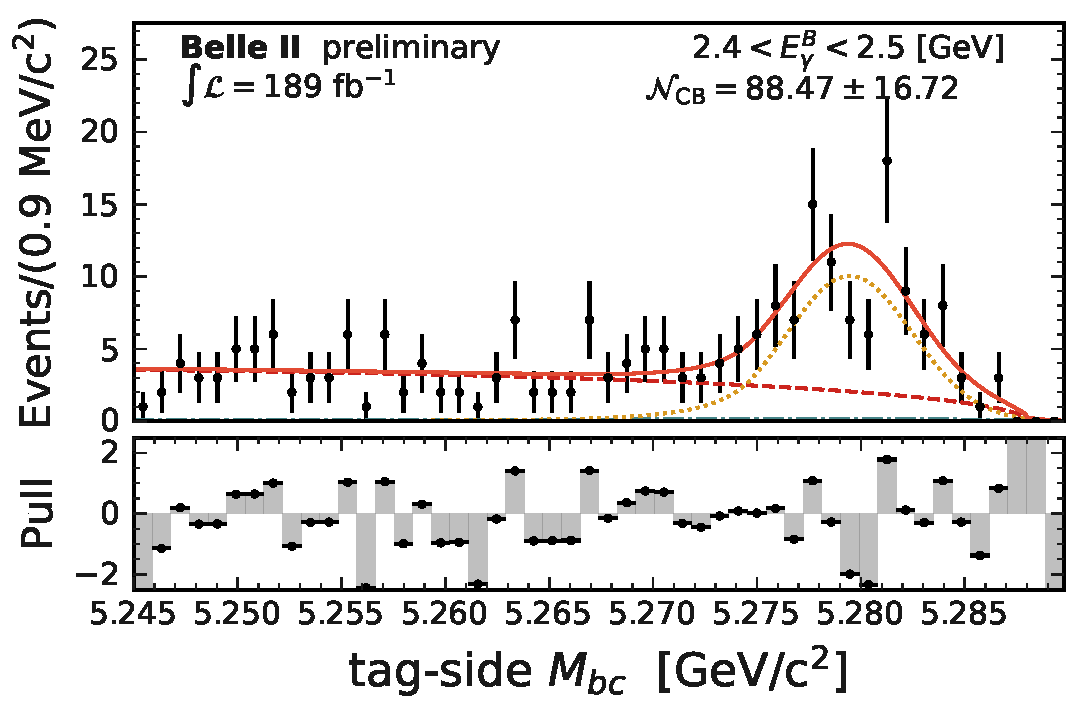
\includegraphics[width=0.3\textwidth]{figures/final_results/data_fits/DATA_MbcFit_2p4to2p5ppdf.pdf}
    }
    \subcaptionbox{\label{fig:data_fit_2p5_2p6}}{
        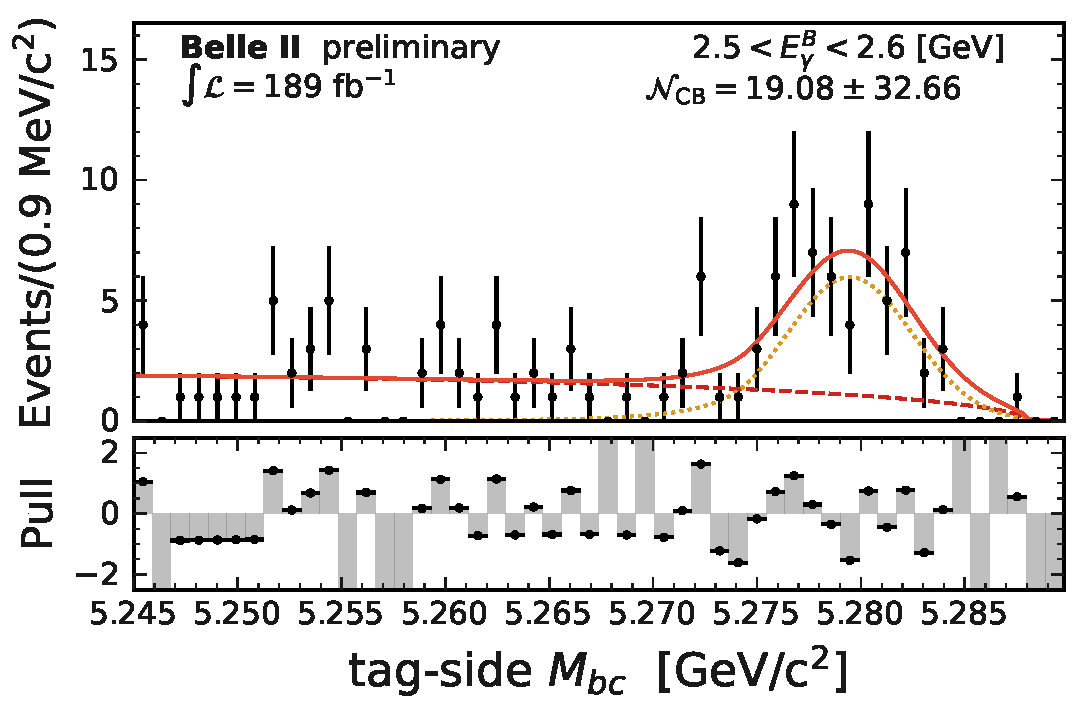
\includegraphics[width=0.3\textwidth]{figures/final_results/data_fits/DATA_MbcFit_2p5to2p6ppdf.pdf}
    }
    \subcaptionbox{\label{fig:data_fit_2p6_2p7}}{
        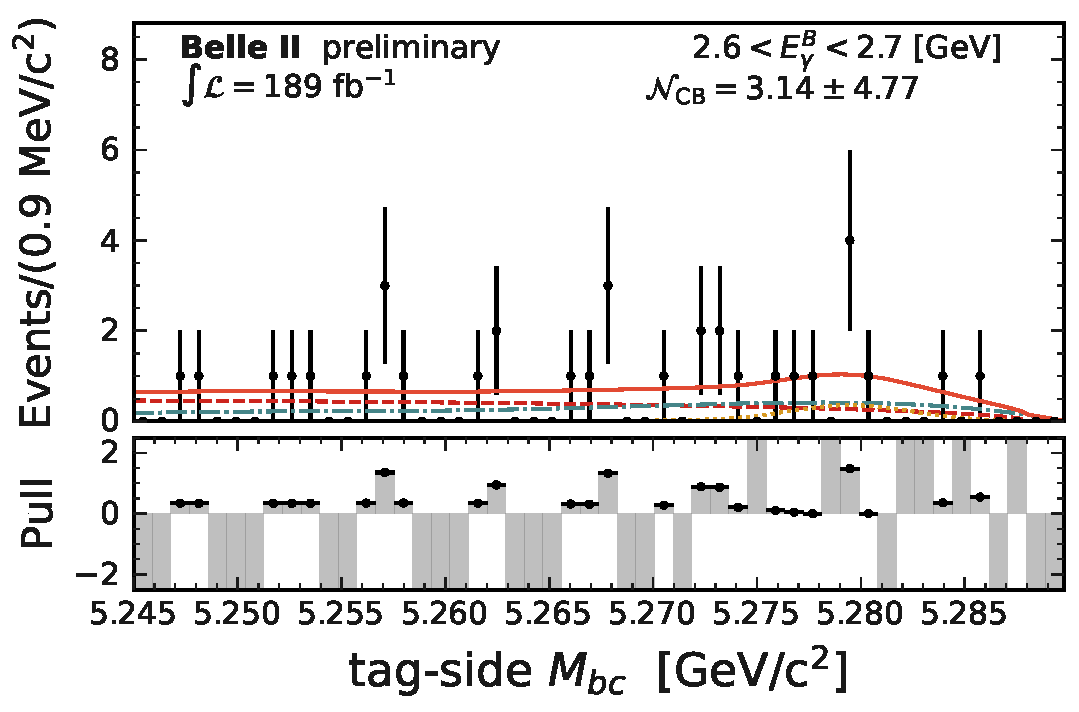
\includegraphics[width=0.3\textwidth]{figures/final_results/data_fits/DATA_MbcFit_2p6to2p7ppdf.pdf}        
    }
    \caption{\label{fig:data_fits_signal}
    Signal region fits.
    }
\end{figure}


\begin{figure}[htbp!]
    \centering
    \subcaptionbox{\label{fig:nosignal_fit_1p8_2p0}}{
        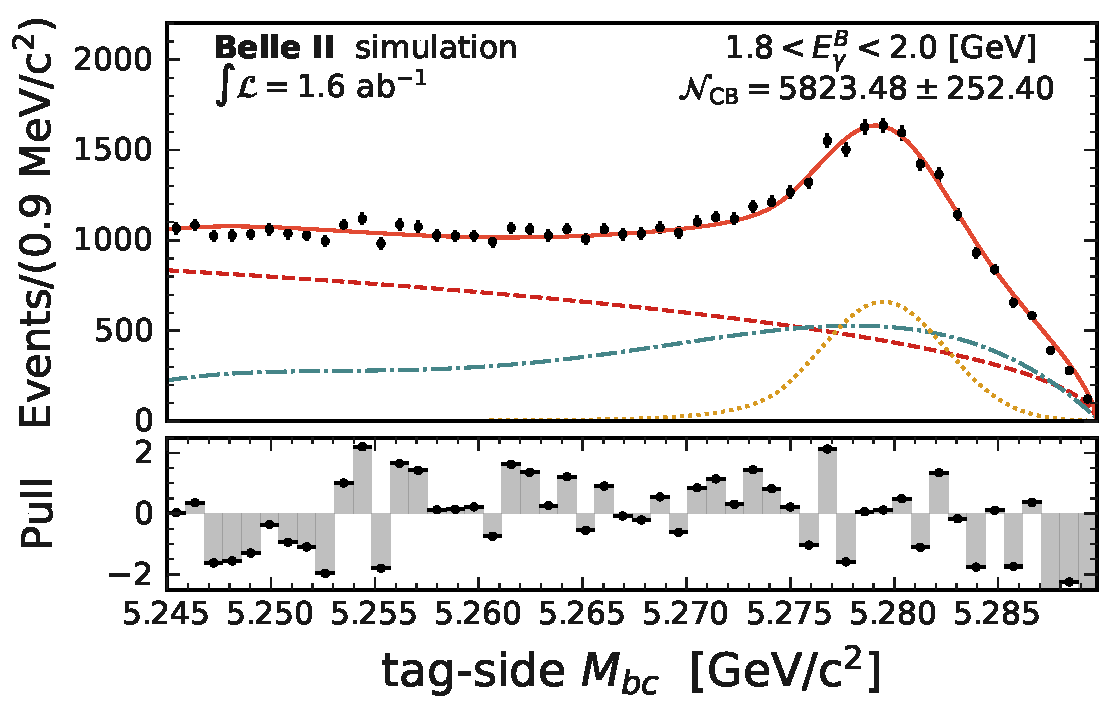
\includegraphics[width=0.3\textwidth]{figures/final_results/mc_fits/NOSIGNALMC_MbcFit_1p8to2p0ppdf.pdf}
    }
    \subcaptionbox{\label{fig:nosignal_fit_2p0_2p1}}{
        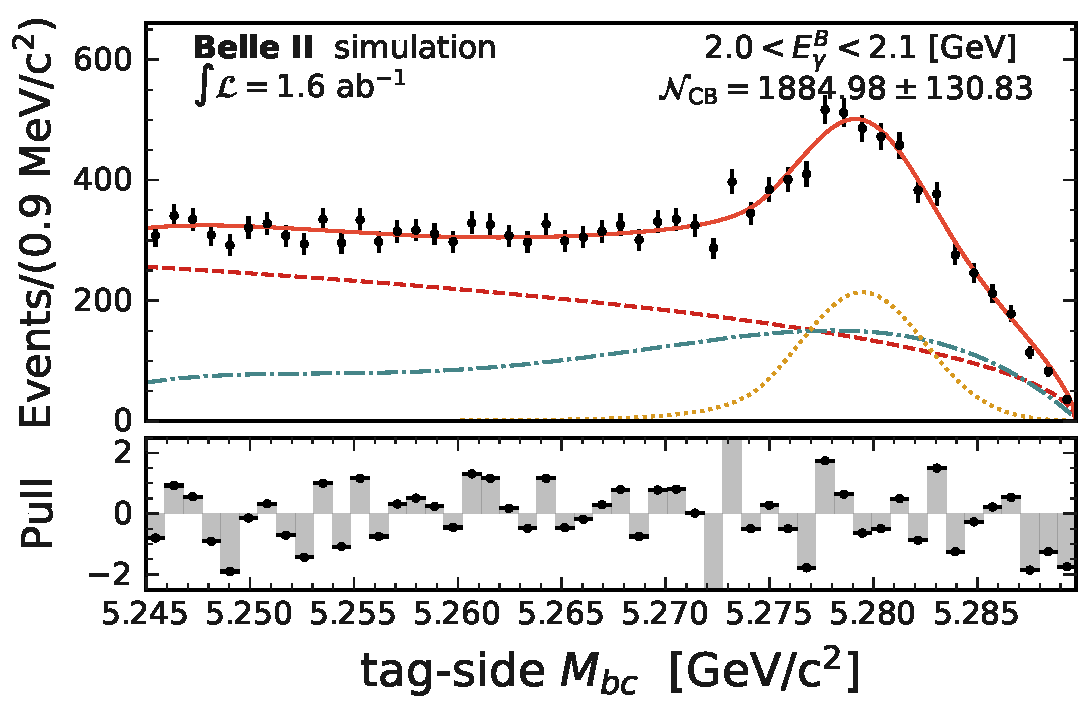
\includegraphics[width=0.3\textwidth]{figures/final_results/mc_fits/NOSIGNALMC_MbcFit_2p0to2p1ppdf.pdf}
    }
    \subcaptionbox{\label{fig:nosignal_fit_2p1_2p2}}{
        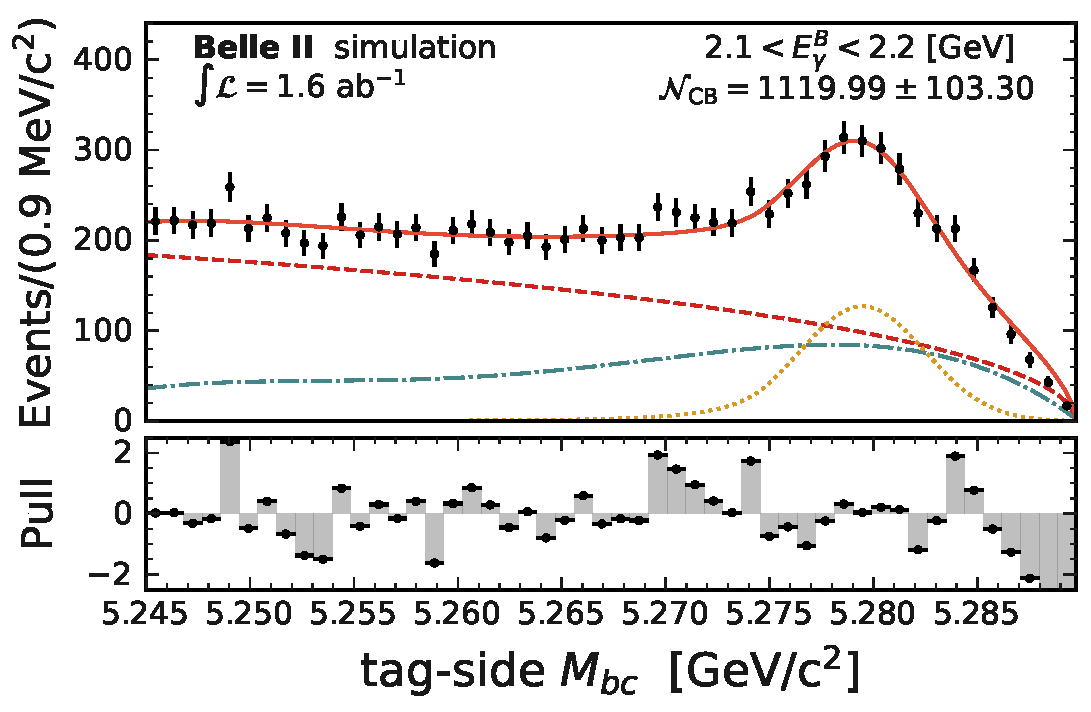
\includegraphics[width=0.3\textwidth]{figures/final_results/mc_fits/NOSIGNALMC_MbcFit_2p1to2p2ppdf.pdf}
    }
    \subcaptionbox{\label{fig:nosignal_fit_2p2_2p3}}{
        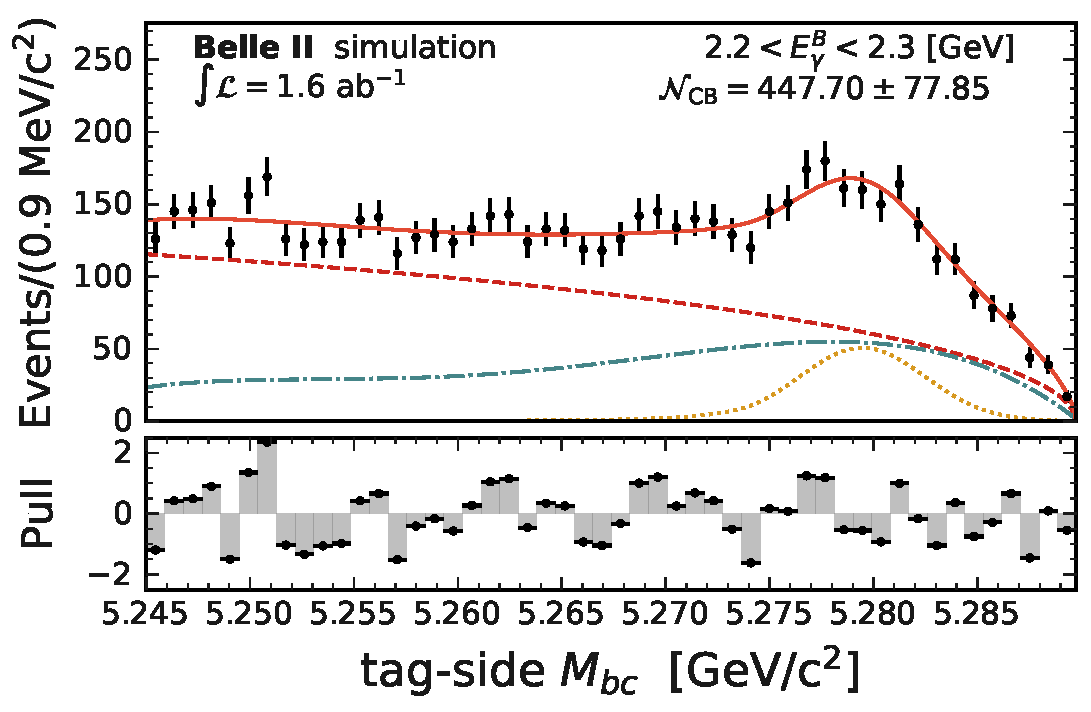
\includegraphics[width=0.3\textwidth]{figures/final_results/mc_fits/NOSIGNALMC_MbcFit_2p2to2p3ppdf.pdf}        
    }
    \subcaptionbox{\label{fig:nosignal_fit_2p3_2p4}}{
        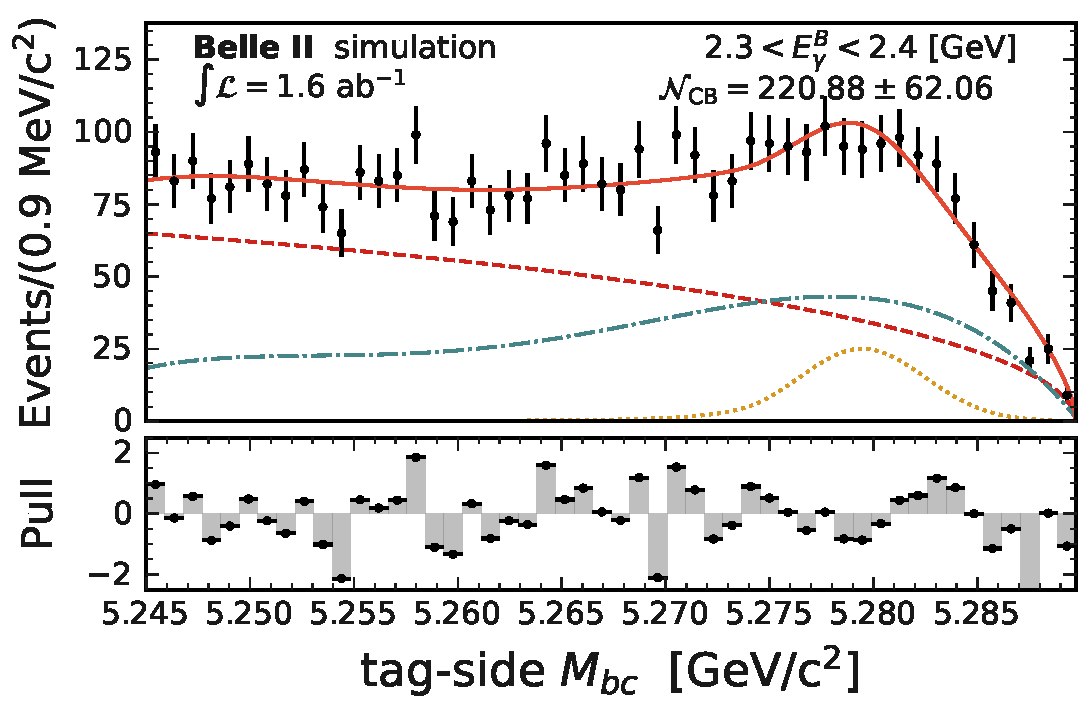
\includegraphics[width=0.3\textwidth]{figures/final_results/mc_fits/NOSIGNALMC_MbcFit_2p3to2p4ppdf.pdf}
    }
    \subcaptionbox{\label{fig:nosignal_fit_2p4_2p5}}{
        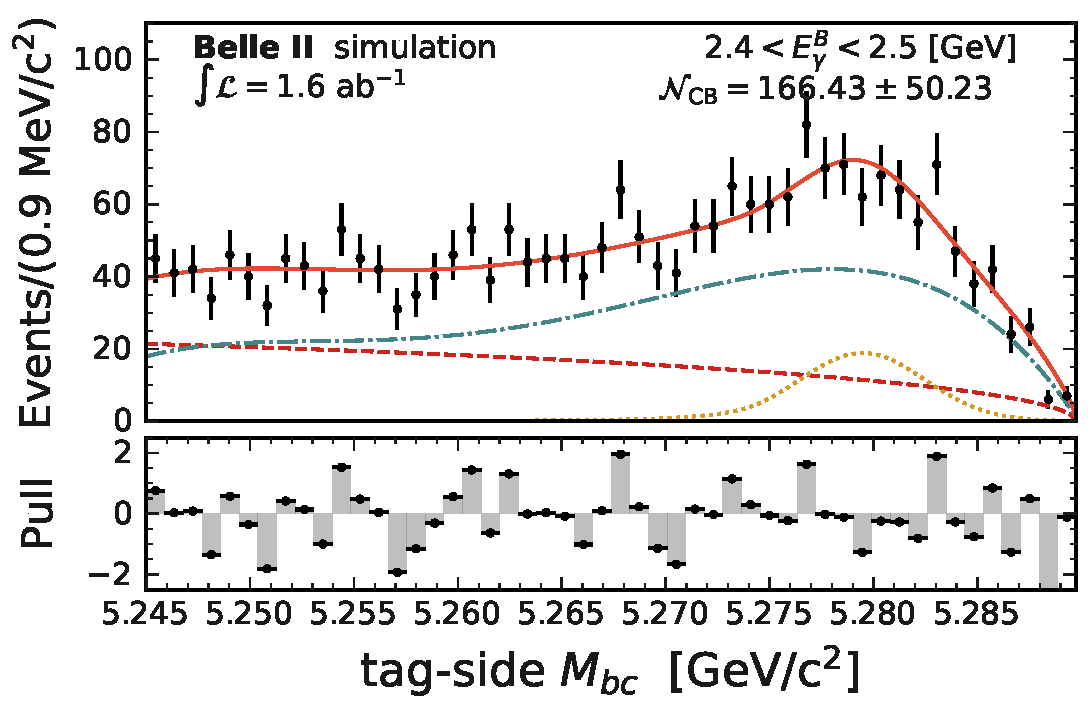
\includegraphics[width=0.3\textwidth]{figures/final_results/mc_fits/NOSIGNALMC_MbcFit_2p4to2p5ppdf.pdf}
    }
    \subcaptionbox{\label{fig:nosignal_fit_2p5_2p6}}{
        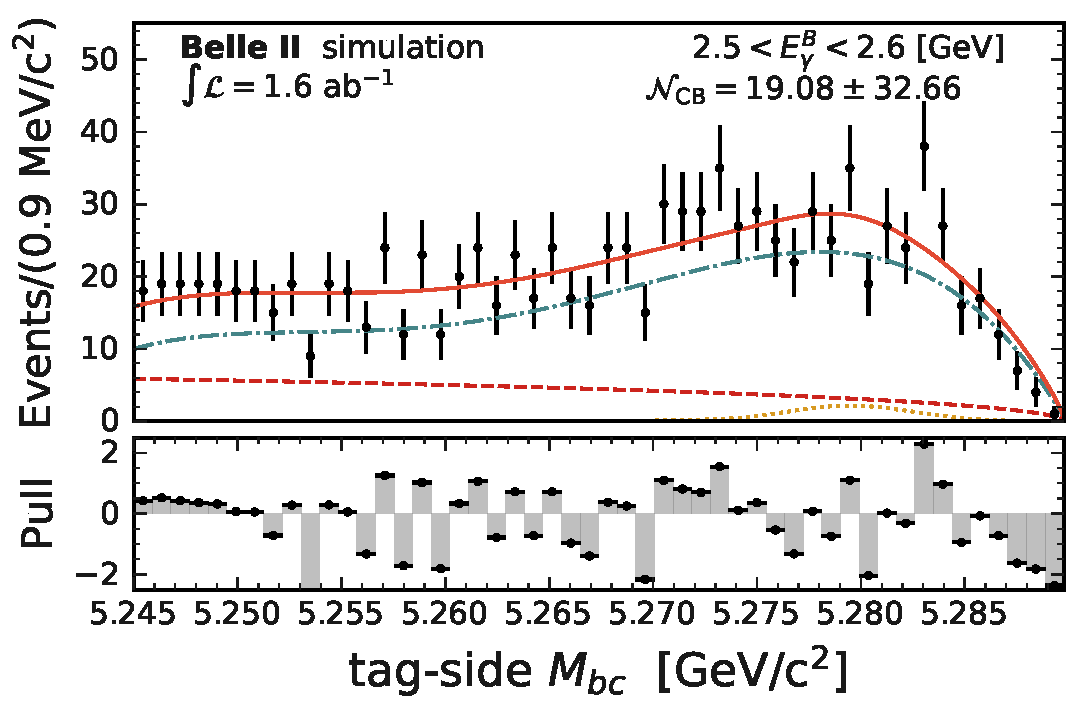
\includegraphics[width=0.3\textwidth]{figures/final_results/mc_fits/NOSIGNALMC_MbcFit_2p5to2p6ppdf.pdf}
    }
    \subcaptionbox{\label{fig:nosignal_fit_2p6_2p7}}{
        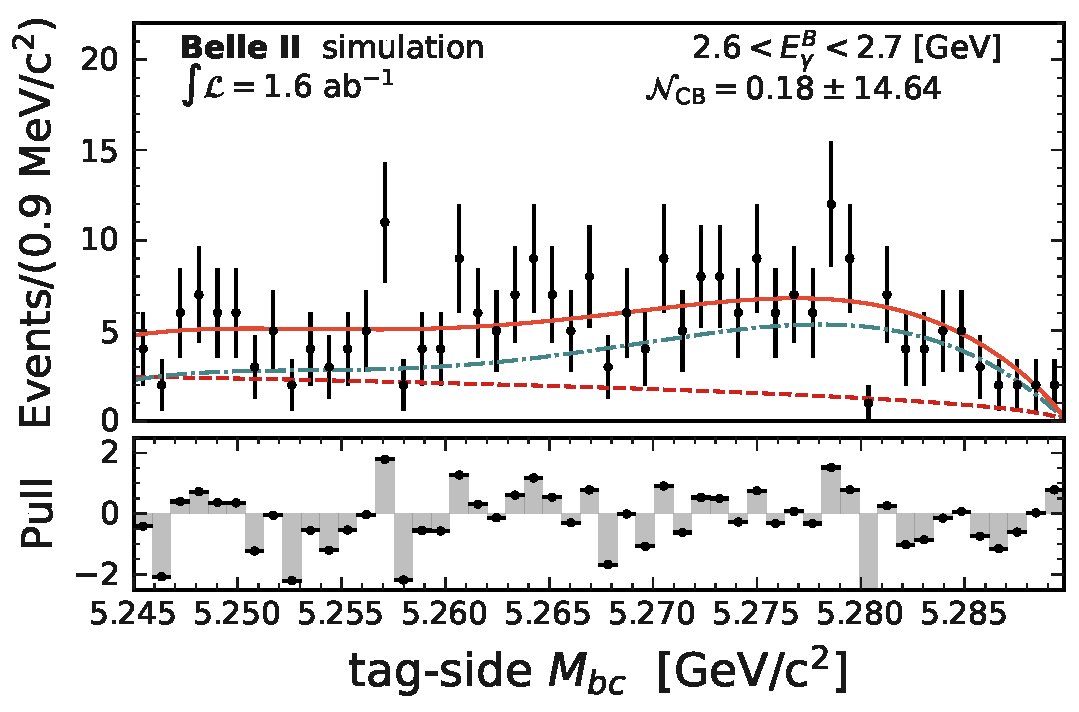
\includegraphics[width=0.3\textwidth]{figures/final_results/mc_fits/NOSIGNALMC_MbcFit_2p6to2p7ppdf.pdf}        
    }
    \caption{\label{fig:nosignal_fits_signal}
    nosignal region fits.
    }
\end{figure}